\section{Membuka SQL Command Atau CLI}
Setelah database telah disiapkan dan direlasikan kita akan membuat query setiap tabel, pertama tama buka kembali aplikasi ORACLE APEX Online anda lalu pilih SQL Workshop.
\begin{itemize}
    \item[1] Buka SQL Workshop pada Oracle Apex Online Anda,lihat Gambar 4.1.
    \item[2] Buka SQL Command pada Oracle Apex Online Anda,lihat Gambar 4.2.
    \item[3] Anda akan menjumpai seperti CLI Database, disitu anda akan membuat query yang nanti akan dijelaskan pada buku ini, lalu pada tab bawah amda akan menjumpai :
    \par Results (Untuk Hasil Dari Query), Explain (Adalah Penjelasan Jika Query Salah), Describe (Untuk Describe Sebuah Objek), Saved SQL (Me-nampilkan data SQL yangg tersimpan), History (Menampilkan Query Yang Pernah Di Run Sebelumnya),lihat Gambar 4.3.      
\end{itemize}

\begin{figure}
        \begin{center}
        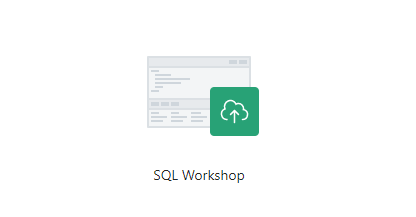
\includegraphics[scale=0.5]{figures/sql_wksp.png}
        \caption{\textit{SQL Workshop}}
        \end{center}
        \end{figure}
        
\begin{figure}
        \begin{center}
        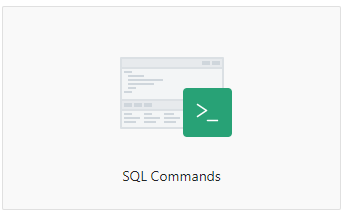
\includegraphics[scale=0.5]{figures/sql_command.png}
        \caption{\textit{SQL Command}}
        \end{center}
        \end{figure}
\begin{figure}
       
        \begin{center}
        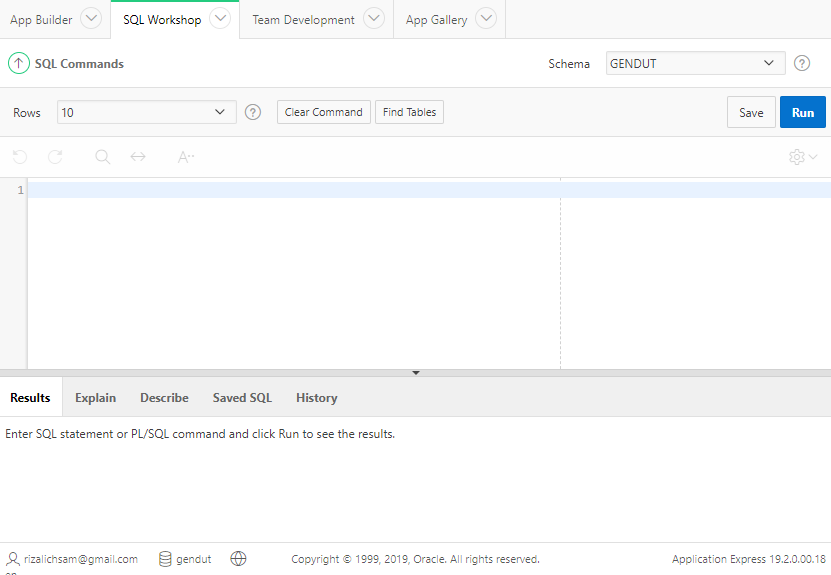
\includegraphics[scale=0.5]{figures/sql_command2.png}
        \caption{\textit{Isi SQL Command}}
        \end{center}
        \end{figure}

\section{Membuat Query}
setelah membuka SQL Command buku ini akan menjelaskan Query dari setiap tabel yang telah direlasikan sebelumnya,berikut adalah penjelasannnya :

\begin{itemize}
    \item Query pada tabel JABATAN\_ORMAWA
            \begin{lstlisting}
/*RUN QUERY PERTAMA*/

CREATE TABLE  "JABATAN_ORMAWA" 
("KODE_JABATAN" NUMBER,
"JABATAN" VARCHAR2(50), 
PRIMARY KEY ("KODE_JABATAN")
USING INDEX  ENABLE
)
/

/*RUN QUERY KEDUA*/

CREATE OR REPLACE EDITIONABLE TRIGGER  "JABATAN_TRG" 
BEFORE INSERT ON JABATAN_ORMAWA 
FOR EACH ROW
BEGIN
  SELECT JABATAN_SEQ.NEXTVAL
  INTO   :new.KODE_JABATAN
  FROM   dual;
END;
/

/*RUN QUERY KETIGA*/

ALTER TRIGGER  "JABATAN_TRG" ENABLE
/
            \end{lstlisting}
    \item Query pada tabel JURUSAN
            \begin{lstlisting}
CREATE TABLE  "JURUSAN" 
   (	"KODE_JURUSAN" NUMBER NOT NULL ENABLE, 
	"NAMA_JURUSAN" VARCHAR2(255) NOT NULL ENABLE, 
	 PRIMARY KEY ("KODE_JURUSAN")
  USING INDEX  ENABLE
   )
/
            \end{lstlisting}
    \item Query pada tabel ORMAWA
            \begin{lstlisting}
CREATE TABLE  "ORMAWA" 
   (	"KODE_ORMAWA" VARCHAR2(255) NOT NULL ENABLE, 
	"NAMA_ORMAWA" VARCHAR2(255) NOT NULL ENABLE, 
	 PRIMARY KEY ("KODE_ORMAWA")
  USING INDEX  ENABLE
   )
/
            \end{lstlisting}
        
        \item Query pada tabel RUANGAN
            \begin{lstlisting}
CREATE TABLE  "RUANGAN" 
   (	"ID_RUANGAN" NUMBER(*,0) NOT NULL ENABLE, 
	"JENIS_RUANGAN" VARCHAR2(255) NOT NULL ENABLE, 
	 PRIMARY KEY ("ID_RUANGAN")
  USING INDEX  ENABLE
   )            
            \end{lstlisting}
\item Query pada tabel STAFF\_BAAK
            \begin{lstlisting}
CREATE TABLE  "STAFF_BAAK" 
   (	"NIK" NUMBER(*,0) NOT NULL ENABLE, 
	"NAMA_STAFF" VARCHAR2(255), 
	"NO_TELP" VARCHAR2(20), 
	"JABATAN" VARCHAR2(30), 
	 PRIMARY KEY ("NIK")
  USING INDEX  ENABLE
   )
/
            \end{lstlisting}
\item Query pada tabel MAHASISWA
            \begin{lstlisting}
/* RUN QUERY PERTAMA */

CREATE TABLE  "MAHASISWA" 
   (	"NPM" NUMBER(*,0) NOT NULL ENABLE, 
	"NAMA" VARCHAR2(255) NOT NULL ENABLE, 
	"KELAS" VARCHAR2(255) NOT NULL ENABLE, 
	"KODE_ORMAWA" VARCHAR2(255) NOT NULL ENABLE, 
	"NO_TELP_MHS" VARCHAR2(14), 
	"KODE_JURUSAN" NUMBER, 
	"KODE_JABATAN" NUMBER, 
	 PRIMARY KEY ("NPM")
  USING INDEX  ENABLE
   )
/

/* RUN QUERY KEDUA */

ALTER TABLE  "MAHASISWA" ADD CONSTRAINT "FK_JABATAN" FOREIGN KEY ("KODE_JABATAN")
	  REFERENCES  "JABATAN_ORMAWA" ("KODE_JABATAN") ENABLE
/

/* RUN QUERY KETIGA */

ALTER TABLE  "MAHASISWA" ADD CONSTRAINT "FK_JURUSAN" FOREIGN KEY ("KODE_JURUSAN")
	  REFERENCES  "JURUSAN" ("KODE_JURUSAN") ENABLE
/

/* RUN QUERY KEEMPAT */

ALTER TABLE  "MAHASISWA" ADD CONSTRAINT "FK_ORMAWA" FOREIGN KEY ("KODE_ORMAWA")
	  REFERENCES  "ORMAWA" ("KODE_ORMAWA") ENABLE
/
            
            \end{lstlisting}
\item Query pada tabel PEMINJAMAN\_RUANGAN
            \begin{lstlisting}
/* RUN QUERY PERTAMA */

CREATE TABLE  "PEMINJAMAN_RUANGAN" 
   (	"ID_PEMINJAMAN" NUMBER GENERATED ALWAYS AS IDENTITY MINVALUE 1 MAXVALUE 999999999999 INCREMENT BY 1 START WITH 1 CACHE 20 NOORDER  NOCYCLE  NOKEEP  NOSCALE  NOT NULL ENABLE, 
	"NPM" NUMBER, 
	"ID_RUANGAN" NUMBER, 
	"NIK" NUMBER, 
	"TANGGAL" DATE, 
	"JAM_AWAL" VARCHAR2(4000), 
	"JAM_AKHIR" VARCHAR2(4000), 
	"STATUS_PEMINJAMAN" VARCHAR2(4000), 
	 PRIMARY KEY ("ID_PEMINJAMAN")
  USING INDEX  ENABLE
   )
/
/* RUN QUERY KEDUA */

ALTER TABLE  "PEMINJAMAN_RUANGAN" ADD CONSTRAINT "FK_NIK" FOREIGN KEY ("NIK")
	  REFERENCES  "STAFF_BAAK" ("NIK") ENABLE
/
/* RUN QUERY KETIGA */

ALTER TABLE  "PEMINJAMAN_RUANGAN" ADD CONSTRAINT "FK_NPM" FOREIGN KEY ("NPM")
	  REFERENCES  "MAHASISWA" ("NPM") ENABLE
/

/* RUN QUERY KEEMPAT */

ALTER TABLE  "PEMINJAMAN_RUANGAN" ADD CONSTRAINT "FK_RUANGAN" FOREIGN KEY ("ID_RUANGAN")
	  REFERENCES  "RUANGAN" ("ID_RUANGAN") ENABLE
/
            
            \end{lstlisting}

\end{itemize}
